\documentclass[12pt,letter]{article}

\usepackage{amsmath}
\usepackage{hyperref}
\usepackage{graphicx}
\usepackage{verbatim}
\usepackage{listings}
\lstset{%
    basicstyle=\scriptsize\ttfamily, %
    language=Matlab, %
    keywordstyle=\color{blue},%
    commentstyle=\color{green!50!black},%
    numberstyle=\color{gray},%
    stringstyle=\color{magenta!70!blue},%
    deletekeywords={type},%
    otherkeywords={xlim,ylim,ones},%
    numbers=left,%
    showstringspaces=false,%
}

\usepackage{tikz}

\tikzstyle{block}=[rectangle,draw=black,thick,minimum size=1.2cm]
\tikzstyle{signal}=[rectangle,text width=1.0cm]
\tikzstyle{junction}=[circle,fill=black,draw=black,inner sep=0,minimum size=1.0mm]
\tikzstyle{operator}=[circle,draw=black,thick,inner sep=2pt]

\newcommand{\ts}[1]{\textsuperscript{#1}}
\newcommand{\rpref}[1]{\ref{#1} on page \pageref{#1}}

\title{ECE480A3 Project Final Report: \\ Diagnosis of Cardiac Arrhythmias from 
Electrocardiography Data}
\author{Robby Stokoe}
\date{\today}

\begin{document}
\maketitle

\begin{abstract}
    The diagnosis of cardiac arrhythmias can be a tedious process when done by
    hand and could benefit greatly from computer automation.  To this end, an 
    algorithm was developed to distinguish between normal heart beats and
    abnormal arrhythmic beats in an ECG waveform.  First an algorithm was
    developed to find the location of QRS complexes in the ECG waveform.
    Principal component analysis was performed using the area around the QRS 
    complex.  20 of the resulting principal components were used to train a
    simple linear classifier to distinguish between normal and abnormal beats.
    The QRS detection algorithm performed very well with x\% false negatives and
    y\% false positives.  The classification algorithm did not fare quite as 
    well with and x\% false positive rate and y\% false negative rate.  More
    sophisticated signal processing techniques could be applied to improve these
    numbers, but the algorithm is good starting point.  
\end{abstract}

\section{Introduction} 
Cardiac arrhythmias are a relatively common set of diseases, affecting 3.4\% of
people in the US \cite{cdc95}.  Diagnosis is done by eye from an ECG trace which
can be tedious.  A common diagnostic technique is to record ECG data from a
patient constantly as they go about normal activity.  This results in a very
long recording which may contain only a few abnormal beats.  An algorithm-driven
diagnosis could potentially eliminate this tedium and also the possibility of
human error if the algorithm is robust enough.  Such an algorithm could be used
in AEDs, pacemakers, or EEG machines.  Even if the algorithm is not as robust as
human diagnosis, it could still assist diagnosis by flagging potentially
abnormal beats for further analysis, allowing a trained cardiologist to quickly
zero-in on the relevant beats.  This project attempts to develop such an
algorithm using signal processing and classification techniques.  

\section{Data}
The data used to develop the signal processing algorithm and train the
classifier were obtained from the MIT-BIH Arrhythmia Database which is available
on \url{physionet.org}.  The data and techniques used to obtain it are described
as follows: 
\begin{quotation}
     The MIT-BIH Arrhythmia Database contains 48 half-hour excerpts of
     two-channel ambulatory ECG recordings, obtained from 47 subjects studied by
     the BIH Arrhythmia Laboratory between 1975 and 1979. Twenty-three
     recordings were chosen at random from a set of 4000 24-hour ambulatory ECG
     recordings collected from a mixed population of inpatients (about 60\%) and
     outpatients (about 40\%) at Boston's Beth Israel Hospital; the remaining 25
     recordings were selected from the same set to include less common but
     clinically significant arrhythmias that would not be well-represented in a
     small random sample.

     The recordings were digitized at 360 samples per second per channel with
     11-bit resolution over a 10 mV range. Two or more cardiologists
     independently annotated each record; disagreements were resolved to obtain
     the computer-readable reference annotations for each beat (approximately
     110,000 annotations in all) included with the database.
\end{quotation}

The data and annotations will be instrumental in training and testing the
classification algorithm.  Figure \ref{fig:raw} shows a portion of a recording
from the Database with annotations showing normal beats, an atrial premature
beat (A) and a premature ventricular contraction (V).  

\section{Algorithm}
The first step of the algorithm will be to identify the locations of QRS
complexes in the ECG.  This will be done by the Pan-Tompkins algorithm shown
schematically in Figure \ref{fig:pan}.  This algorithm works by differentiating
the signal, squaring the derivative, and then comparing the resulting squared
derivative with some threshold.  The location of the maximum absolute value of
the signal where the squared derivative is above the threshold is taken to be
the location of the R-wave in the QRS complex \cite{pan-tompkins85}

\begin{figure}[hbtp]
    \centering
    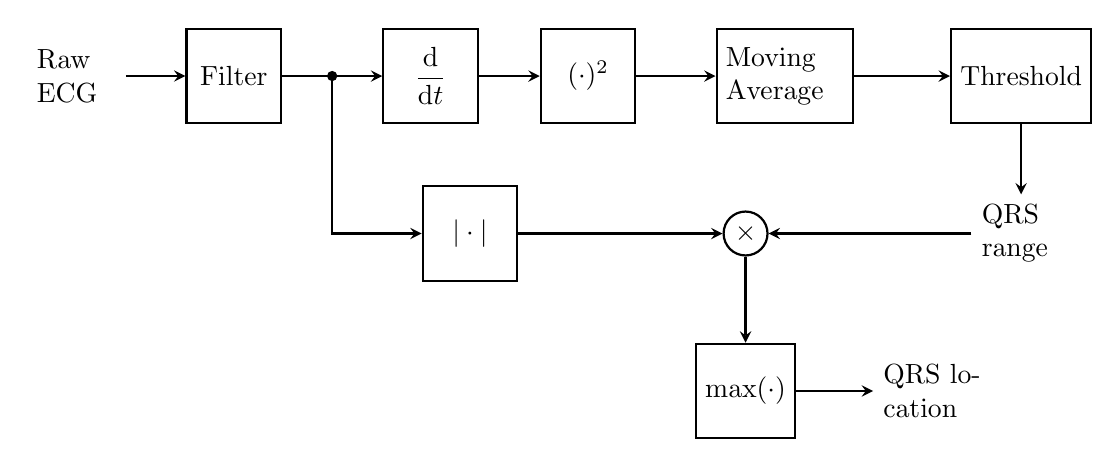
\begin{tikzpicture}[thick,>=stealth]
        \node[signal] (input) at (-6.5,0) {Raw ECG};
        \node[block] (filter) at (-4.5,0) {Filter};
        \node[block] (deriv)  at (-2,0) 
            {$\displaystyle\frac{\mathrm{d}}{\mathrm{d}t}$};
        \node[block] (square) at (0,0)  {$(\cdot)^2$};
        \node[block] (thresh) at (5.5,0) {Threshold};
        \node[signal] (range) at (5.5,-2)  {QRS range};
        \node[block,text width=1.5cm] (avg) at (2.5,0) {Moving Average};
        \node[block] (abs) at (-1.5,-2) {$|\cdot|$};
        \node[operator] (mult) at (2.0,-2) {$\times$};
        \node[block] (max) at (2.0,-4) {$\max(\cdot)$};
        \node[signal,text width=1.5cm] (location) at (4.5,-4) {QRS location};

        \draw [->] (input) -- (filter);
        \draw [->] (filter) -- node[junction] (branch) {} (deriv.west);
        \draw [->] (deriv) -- (square);
        \draw [->] (square) -- (avg);
        \draw [->] (avg) -- (thresh);
        \draw [->] (thresh) -- (range);
        \draw [->] (range) -- (mult);
        \draw [->] (mult) -- (max);
        \draw [->] (branch) |- (abs);
        \draw [->] (abs) -- (mult);
        \draw [->] (max) -- (location);
    \end{tikzpicture}
    \caption{The Pan-Tompkins Algorithm for Finding QRS Complexes}
    \label{fig:pan}
\end{figure}

Once the location of the center of the QRS complex is determined, the portion of
the signal few hundred milliseconds before and after the QRS complex is
extracted for analysis.  To train the classifier, a multitude of these signal
excerpts were gathered and sorted by normal \textit{vs.} abnormal rhythm.
Principal component analysis was performed on this entire data set to obtain a
transformation to be used for classification.  Only some of the components of
this transformation were used to simplify classification.  To obtain the best
discrimination between normal and abnormal beats, the components for which the
mean values of the normal and abnormal beats were the most significantly
different were used.  In addition to the principal components, the R-R interval
for each beat was also found and used as an additional component.  

\section{Implementation}
The algorithm was implemented in MATLAB.  All code used is included in the
appendix and available on github at
\url{https://github.com/robbystk/Arrythmias}. The first step was to download ECG
data and annotations from Physionet using the \verb`rdsamp()` and \verb`rdann()`
functions from Physionet's WFDB toolbox as follows: 
\begin{verbatim}
[tm,sig] = rdsamp(url,1);
[ann,type,subtype,chan,num,comments] = rdann(url,'atr');
\end{verbatim}
Where \verb`url` is the Physionet URL from which to download the data, e.g\@.
\verb`'mitdb/100'`.  These lines were wrapped in a function to make them easier
to use.  See page \pageref{fun:fetch} for the full function.  Figure
\ref{fig:raw} shows an example of ECG data directly from physionet with beat
annotations.  The annotations do not always correspond directly with the
location of the QRS complex because they correspond to the entire beat rather
than a specific feature.  So the next step is to determine the exact location of
the QRS complexes.  

\begin{figure}[hbtp]
    \centering
    \includegraphics[height=0.44\textheight]{../figures/figures_01}
    \caption{Examples of Raw ECG Signals Showing Normal Beats (N), an Atrial
    Premature Beat (A), and Premature Ventricular Contraction (V)}
    \label{fig:raw}
\end{figure}

The first step in the Pan-Tomkins alorithm is to filter the signal.  This was
done by a fourth-order Butterworth bandpass filter with cutoffs at 1 and 50Hz, 
as well as a notch filter at 60Hz.  The full implementation is shown in the
\verb`filterecg()` function in section \rpref{fun:filter}.  The effect of this
filter on an ECG signal is shown in Figure \ref{fig:filter}.  The rest of the
QRS-detection algorithm was implemented in the function \verb`findqrs()` shown
in section \rpref{fun:qrs}.  Figure \ref{fig:qrs} shows an example of the
signals at each stage of the algorithm.  

\begin{figure}[hbtp]
    \centering
    \includegraphics[height=0.44\textheight]{../figures/figures_02}
    \caption{The Effect of \texttt{filterecg()} on an ECG Signal}
    \label{fig:filter}
\end{figure}

\begin{figure}[hbtp]
    \centering
    \includegraphics[height=0.44\textheight]{../figures/figures_03}
    \caption{Example Signals at the Various Stages of the Pan-Tompkins
    QRS-Detection Algorithm}
    \label{fig:qrs}
\end{figure}

It was decided to distinguish A form normal because
reasons (mostly I'm a dumbass) Here's some plots and shit.  

The ease of distinguishing an arrhythmia with DSP depends on the particular
arrhythmia.  During research, an arrhythmia will be chosen that should be
possible to distinguish using elementary signal processing techniques including
IIR filtering, adaptive filtering, wavelet transforms, and frequency-domain
analysis.  

\section{Results}

\section{Conclusion}

\appendix
\section{Matlab Code}
\subsection{\texttt{fetch()}}
\label{fun:fetch}
\lstinputlisting{../matlab/fetch.m}
\subsection{\texttt{filterecg()}}
\label{fun:filter}
\lstinputlisting{../matlab/filterecg.m}
\subsection{\texttt{findqrs()}}
\label{fun:qrs}
\lstinputlisting{../matlab/findqrs.m}
\subsection{\texttt{crop()}}
\label{fun:crop}
\lstinputlisting{../matlab/crop.m}
\subsection{\texttt{pca\_transform()}}
\label{fun:pca}
\lstinputlisting{../matlab/pca_transform.m}
\subsection{\texttt{plotpca()}}
\label{fun:plotpca}
\lstinputlisting{../matlab/plotpca.m}
\subsection{\texttt{plotecg()}}
\label{fun:plotecg}
\lstinputlisting{../matlab/plotecg.m}
\subsection{\texttt{texify()}}
\label{fun:tex}
\lstinputlisting{../matlab/texify.m}
\subsection{\texttt{gather.m}}
\label{scr:gather}
\lstinputlisting{../matlab/gather.m}
\subsection{\texttt{figures.m}}
\label{scr:figures}
\lstinputlisting{../matlab/figures.m}
\subsection{\texttt{train.m}}
\label{scr:train}
\lstinputlisting{../matlab/train.m}

\bibliography{sources}
\bibliographystyle{IEEEtran}

\end{document}
